%\begin{savequote}[75mm]
% The idea that complex physical, biological or sociological systems can be exactly described by a few formulae is patently absurd. The construction of idealized representations that capture important stable aspects of such systems is, however, a vital part of general scientific analysis...
%\qauthor{Sir David Cox}
%\end{savequote}

\chapter{Background}
This chapter lays the foundation for those that follow by introducing 
the essential toolkit of probabilistic modeling: the language of 
generative models, the building blocks of time series, and the algorithms
of Bayesian inference. 


\section{Generative Probabilistic Models}
\label{sec:generative_models}
Generative probabilistic models formalize a story of how data comes to be. 
While this story never captures every physical detail, it serves as an 
idealized version that captures the essence of the system. For example, when
modeling a neural spike train, we will ignore the states of individual ion 
channels and the nonlinear dynamics of membrane potential and instead 
characterize the instantaneous \emph{firing rate} of a neuron --- the 
probability that a neuron spikes at any moment in time. 

As a simple illustration, consider the following generative
process. Suppose a neuron has two states, an \emph{up} state and an
\emph{down} state. In the \emph{up} state, the neuron spikes at a high
rate, say 100Hz, and in the \emph{down} state it rarely fires, say at 1Hz.
Assume that every 50ms the neuron flips a coin to decide what state it
will be in, and then fires a random number of spikes according to the
rate associated with its current state. Once 50ms have elapsed, it
flips another coin and its rate immediately changes to reflect its new
state. Moreover, assume that all we observe is the number of spikes
fired in each 50ms time bin.  Our goal is to infer the latent state of
the neuron given the observed spike counts.

\begin{figure}[t]
\centering%
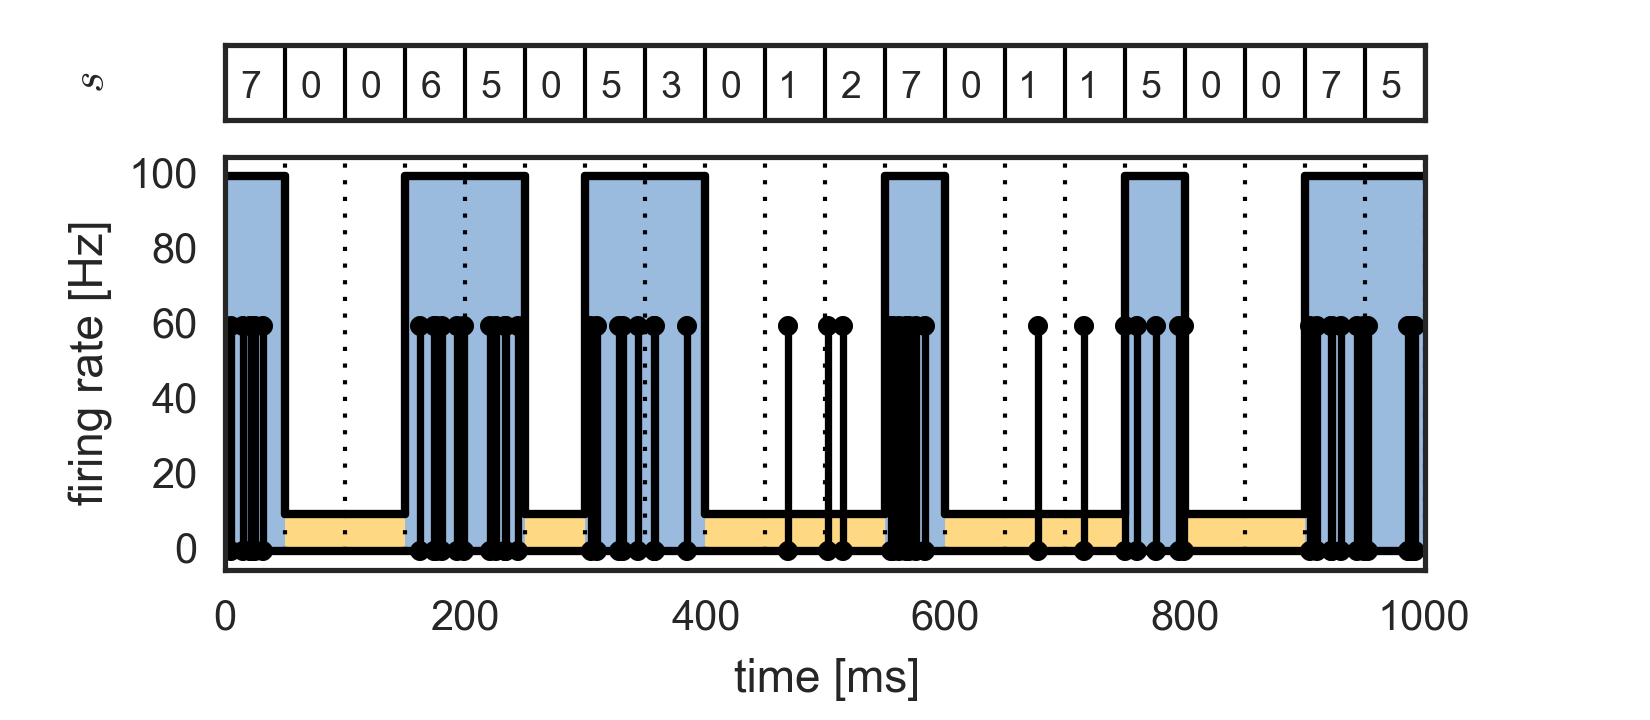
\includegraphics[width=5.5in]{figures/ch1/figure1} 
\caption[Simple neuron with two states]{A simple neuron that randomly switches between an \textit{up} and a \textit{down} state every 50ms. Each state has an associated firing rate from which a Poisson number of spikes are drawn.}
\label{fig:updown}
\vspace{-0.5cm}
\end{figure}


Clearly, this generative story contains many simplifying assumptions
and omits a great amount of detail. In addition to assuming that
spiking is adequately captured by firing rates, the notion that a
neuron has only two firing rates and that it randomly switches between
them is obviously a gross simplification. Nevertheless, this very
simple model captures some patterns of spiking that have been observed
in experiment \cite{cowan1994spontaneous, shu2003turning}. 

\sloppy We can formalize this generative story with a probabilistic
model that specifies a distribution over latent states and
observed spike counts. Let~$s_t \in \naturals$ denote the number of
spikes counted in the~$t$-th time bin,
and~$z_t \in \{\textit{up}, \textit{down}\}$ denote the corresponding
state of the neuron. The assumption that states are drawn from a coin
flip corresponds to the prior distribution,
${z_t \sim \distBernoulli(\rho)}$, where~$\rho$ specifies the
probability of \textit{up} versus \textit{down} states.  Implicitly,
we assumed that~${\rho=\tfrac{1}{2}}$, though this need not be the
case.  We previously said that the neurons fire a random number of
spikes according to their state-dependent firing rate; now we will
formalize this by
assuming,~${s_{t} \sim \distPoisson(\lambda_{z_t} \cdot \Delta t)}$,
where ${\Delta t = 0.05\text{s}}$,
${\lambda_{\textit{up}} = 100\,\text{spikes/s}}$, and
${\lambda_{\textit{down}} = 10\,\text{spike/s}}$. 
The likelihood is,
\begin{align}
  \label{eq:lkhd_chain_rule}
  %p(\bs, \bz \given \rho, \lambda_{\textit{up}}, \lambda_{\textit{down}}, \Delta t) 
  %&= p(\bz \given \rho) \, p(\bs \given \bz, \lambda_{\textit{up}}, \lambda_{\textit{down}}, \Delta t) \\
  p(\bs, \bz \given \rho, \blambda, \Delta t) 
  &= p(\bz \given \rho) \, p(\bs \given \bz, \blambda, \Delta t) \\
  \label{eq:lkhd_factorized}
  &= \prod_{t=1}^T p(z_t \given \rho) \, p(s_t \given \lambda_{z_t}, \Delta t) \\
  &= \prod_{t=1}^T \distBernoulli(z_t \given \rho) \, \distPoisson(s_t \given \lambda_{z_t} \cdot \Delta t).
\end{align} 
Here, we have introduced notation that will be used throughout this
thesis. Bold symbols like~$\bs$ will denote arrays of
random variables. Typically, lowercase bold symbols will denote
vectors, as in this case,~${\bs = \big[s_1, \ldots, s_T \big]}$ 
and~${\blambda = \big[ \lambda_{\textit{up}}, \lambda_{\textit{down}} \big]}$.

In addition to specifying functional forms for the distributions,
${p(z_t \given \rho)}$ and~${p(z_t \given \lambda_{z_t}, \Delta t)}$,
the probabilistic model also formalizes the particular factorization of
the likelihood implied by the generative story.
Eq.~\ref{eq:lkhd_chain_rule} simply applies the chain rule of
probability, which does not reflect any loss of generality. However,
in going from \eqref{eq:lkhd_chain_rule} to
\eqref{eq:lkhd_factorized}, we have asserted that the latent
states~$z_t$ and~$z_{t'}$ are conditionally independent given~$\rho$,
and that the spike counts~$s_{t}$ and~$s_{t'}$ are conditionally
independent given their corresponding latent states. This conditional
independence assumption, which was implicit in the generative story,
is made explicit when we factor the likelihood into a product
over time bins. When we hypothesize relationships between different variables,
we are making assertions about the factorization of the likelihood. 
In Section~\ref{sec:motifs}, different patterns of conditional dependence 
that form the building blocks of models for dynamic data.

% Prior distributions on parameters
\subsubsection{Conjugate Prior Distributions}
The model above assumes that the firing rates are known, but in practice 
this is a bit unreasonable. A more reasonable hypothesis is that neurons have 
two firing rates, and while we do not know their exact values, we can 
specify a distribution over them. Similarly, we may not know 
the exact probability of each state,~$\rho$, but perhaps we can say
that it should not be too close to zero or one, with a mean of 0.5.
When crafting a probabilistic model, we can express these prior
intuitions and simultaneously make inference a bit easier by using
\emph{conjugate} prior distributions.


%Intuitively, a prior distribution is conjugate with the likelihood
%if the conditional distribution has the same form.
For example,
take the parameter,~$\lambda_{\textit{up}}$. If we look at the
likelihood as a function of~$\lambda_{\textit{up}}$ and ignore
terms that do not depend on this parameter, we have,
\begin{align}
  p(\bs, \bz \given \rho, \blambda, \Delta t)
  &\propto \prod_{t=1}^T \left[
    \distPoisson(s_t \given \lambda_{\textit{up}} \cdot \Delta t)
    \right]^{\bbI[z_t = \textit{up}]} \\
  &\propto \prod_{t=1}^T \left[
    \lambda_{\textit{up}}^{s_t} \,
    e^{-\lambda_{\textit{up}} \cdot \Delta t}
    \right]^{\bbI[z_t = \textit{up}]} \\
  &=
  \lambda_{\textit{up}}^{s_{\textit{up}}} \,
  e^{-\lambda_{\textit{up}} \cdot t_{\textit{up}}},
\end{align}
where
\begin{align}
  s_{\textit{up}} &= \sum_{t=1}^T s_t \cdot \bbI[z_t = \textit{up}], \\
  t_{\textit{up}} &= \sum_{t=1}^T \Delta t \cdot \bbI[z_t = \textit{up}].
\end{align}

%This likelihood is conjugate with a gamma prior,
Now consider a gamma prior distribution,
\begin{align}
  p(\lambda_{\textit{up}} \given \alpha, \beta)
  &= \distGamma(\lambda_{\textit{up}} \given \alpha, \beta) \\
  &\propto \lambda_{\textit{up}}^{\alpha - 1} \,
  e^{-\lambda_{\textit{up}} \cdot \beta}.
\end{align}
The conditional distribution over~$\lambda_{\textit{up}}$ given the
observed spike counts, the latent states, and the prior is
proportional to the likelihood times the prior. This simplifies to,
\begin{align}
  p(\lambda_{\textit{up}} \given \bs, \bz, \alpha, \beta)
  &\propto p(\bs, \bz \given \rho, \blambda, \Delta t) \,
  p(\lambda_{\textit{up}} \given \alpha, \beta) \\
  &\propto \lambda_{\textit{up}}^{s_{\textit{up}} + \alpha - 1} \,
  e^{-\lambda_{\textit{up}} (t_{\textit{up}} +\beta)} \\
  &\propto \distGamma(\lambda_{\textit{up}} \given
  s_{\textit{up}} + \alpha, \,
  t_{\textit{up}} + \beta).
\end{align}
Since both the prior and the the conditional distribution
over~$\lambda_{\textit{up}}$ are in the gamma family, we say gamma
prior is conjugate with this product-of-Poissons likelihood.
Moreover, the parameters of
conditional distribution only depend on~$\bs$ and ~$\bz$ through
simple \emph{sufficient statistics},~$s_{\textit{up}}$
and~$t_{\textit{up}}$. A beta distribution on the state probability,
~${\distBeta(\rho \given \tau_0, \tau_1)}$, is similarly conjugate
with the product-of-Bernoulli likelihood that links~$\rho$ and~$\bz$.
In fact,
conjugate priors exist for all likelihoods in the \emph{exponential
  family}. These ideas are thoroughly discussed in standard machine
learning and Bayesian statistics textbooks like~\citet{Murphy-2012}.

Putting this all together, we can now write down the \emph{joint
  distribution} of our probabilistic model --- the
product of the likelihood and the prior distributions:
\begin{align}
  \label{eq:full_joint}
  p(\bs, \bz, \rho, \blambda \given \alpha, \beta, \tau_0, \tau_1, \Delta t) 
  &= p(\bs, \bz \given \rho, \blambda, \Delta t) \,
  p(\rho \given \tau_0, \tau_1) \, 
     p(\blambda \given \alpha, \beta).
\end{align}


% Latent variables (states at each time)
% Parameters rates associate with each state
\paragraph{Latent Variables, Parameters, and Hyperparameters}
As our models get increasingly complicated, 
we will often distinguish between the different types of random
variables. The states,~$\bz$, are called \emph{latent
  variables} because their number grows with the size of the dataset,
in this case there is one latent state per time bin. The unknown latent state
probability,~$\rho$, and the firing rates,~$\blambda$, are called
\emph{parameters} because there are a fixed number of them. The
remaining values,~${\{ \alpha, \beta, \tau_0, \tau_1, \Delta t \} }$,
are called \emph{hyperparameters}. These are constants that we set
prior to performing inference.  Typically, these can be tuned
cross-validation, or simply set based on intuition and physical
constraints.

\subsection{Representations of Spike Trains}
% Notation for sets of spike times or spike count matrices
As modelers, one of the first decisions we must make is how we
represent our data. In this thesis we will focus solely on modeling
spike trains, which are sequences of discrete events in time. These
spike trains typically come from spike sorting algorithms applied to
extracellular recordings from multi-electrode arrays
\cite{lewicki1998review}, or from
deconvolution algorithms applied to optically recorded calcium
fluorescence traces \cite{pnevmatikakis2016simultaneous,
  vogelstein2010fast}. Reducing the data to the set of spikes often 
results in an enormous compression. Rather than considering electrode 
potentials, which are often sampled at upwards of 10kHz, or calcium 
fluorescence traces, which are highly autocorrelated due to the relatively 
slow dynamics of calcium concentration in cells, we can instead consider 
only the times of action potentials.

While this thesis treats the spike trains as given, it is also possible to
work directly with the observed extracellular recordings or calcium
fluorescence and treat the spike train as a latent variable.  Then,
the spike train must be inferred along with the rest of the model's
latent variables and parameters, cf. \cite{pillow2013model}. As we just 
mentioned, this will typically incur a substantial cost, but it may be 
worthwhile if there is considerable uncertainty in the spike timing 
and if precise timing is important to the overarching model.

The most general representation of a spike train is as a set of~$M$
\emph{marked} spike times.
Let,
\begin{align}
  \mcS = \left \{ (s_m, c_m) \right \}_{m=1}^M \subset [0, T] \times \{1, \ldots, N\}.
\end{align}
Each member of this set consists of a real-valued spike time~$s_m$ in
the interval~$[0, T]$, and an integer,~$c_m \in \{1, \ldots, N\}$,
that specifies the index of the cell that generated this spike. 
% In the working example of a neuron with an \emph{up} and \emph{down}
% state there is only one neuron ($N=1$), so the cell markers would be
% trivially equal to~$c_m=1$.
This continuous-time representation is
warranted when the temporal resolution of the data is considerably
higher than the timescale of typical action potentials. For example,
multielecrode arrays typically have sampling intervals of~$0.1$ms or
smaller, whereas the width of action potentails is on the order
of~$1$ms. This allows us to specify the spike time as an effectively
real-valued number.  
% Calcium imaging methods typically have much lower temporal
% resolution and are often sampled at lower rates, but by deconvolving
% spike trains it may be possible to obtain effectively higher
% resolution than the raw data affords.

We typically model sets of discrete events like these as realizations
of a \emph{marked point process} \cite{daley2003introduction1}. Such a
process is defined by its firing rates\footnote{In the point process
  literature, these firing rates are called \emph{conditional
    intensity functions}.},
${\{\lambda_n(t \given \mcH_t)\}_{n=1}^N}$, where $\mcH_t$ captures
the history of the process through time~$t$. For example, the history
may include the previous spikes,~${\mcH_t = \{(s_m, c_m): s_m < t\}}$,
or some external covariates,~$x(t)$.  If we consider a small time
window,~${[t, t+\Delta t)}$, and take the limit as~$\Delta t$
approaches zero, the expected number of spikes fired by neuron~$n$ in
the window~${[t, t+\Delta t)}$
is~${\lambda_n(t \given \mcH_t) \cdot \Delta t}$. Our
goal is then to specify flexible and interpretable conditional intensity
functions. Chapter~\ref{chap:hawkes} 

The limiting perspective on the conditional intensity functions
suggestions an alternative, discrete-time representation.  Rather than
modeling a set of continuous spike times and conditional firing rates,
we may instead represent a spike count matrix,~$\bS$, and the
corresponding rate matrix,~$\bLambda$, where,
\begin{align}
  \bS &= 
        \begin{bmatrix}
          s_{1,1} & \cdots & s_{1,N} \\
          & & \\
          \vdots  &        & \vdots  \\ 
          & & \\
          s_{T,1} & \cdots & s_{T,N}
        \end{bmatrix}, 
  & & &
  \bLambda &= 
        \begin{bmatrix}
          \lambda_{1,1} & \cdots & \lambda_{1,N} \\
          & & \\
          \vdots  &        & \vdots  \\ 
          & & \\
          \lambda_{T,1} & \cdots & \lambda_{T,N}
        \end{bmatrix}.
\end{align}
Here,~$s_{t,n} \in \naturals$ denotes the number of spikes fired in
the~$t$-th time bin by the~$n$-th neuron, and~$\lambda_{t,n}$ denotes 
the corresponding firing rate. Sometimes, the effects we
are interested in studying occur at relatively slow time scales, so
discretizing may provide valuable compression while retaining most of
the relevant information. For example, if we are studying neural
dynamics on the order of minutes, then simply knowing how many spikes
occurred each second may provide most of the relevant information, while
precise spike timing may be superfluous.

However, the primary reason to discretize spike times into a matrix of
counts is that the statistics and machine learning community have
developed a much broader set of models for matrices than for sets of
continuous time events.  In the next section, we will explore a number
of common modeling motifs that can be applied to time series data
represented as matrices, and many of the chapters of this thesis will
focus on extending these motifs in novel ways.


\subsection{Motifs of Time Series Models}
\label{sec:motifs}
The art of probabilistic modeling is in balancing conflicting concerns:
our model should capture as much of the relevant structure in the data 
as possible, drawing on our intuition and our existing knowledge of the 
system, yet at the same time we wish to limit the complexity of the model
so that we may perform inference efficiently. One of the ways that we 
accomplish this balancing act is by composing our model out of common,
well-studied motifs. 

\paragraph{Mixture Models}
% Discrete latent states
Our working example from Section~\ref{sec:generative_models}
illustrates one such motif --- a simple mixture model.  The firing
rate takes assumes only two values, and the observed spike counts are
a mixture of counts drawn from the \textit{up} state and counts from
the \textit{down} state. We can easily extend this to populations of
neurons and mixtures of more than two states.  Suppose there are
now~$K$ states, such that~${z_t \in \{1, \ldots, K\}}$. Furthermore,
we generalize the rates~$\lambda_{\textit{up}}$
and~$\lambda_{\textit{down}}$, to vectors of rates, one for each
neuron and state.
Let,~${\blambda_k = \big[ \lambda_{1,k}, \ldots, \lambda_{N,k}\big]}$,
denote a vector of rates where $\lambda_{n,k}$ is the firing rate of
the~${n\text{-th}}$ neuron in state~$k$.  We can write the full rate
matrix,~$\bLambda$, as the outer product of a ~${T \times K}$
indicator matrix,~$\bZ$, and an~${N \times K}$ rate
matrix,~$\bC$. Let~$\be_k$ denote a length-$K$ column vector that is all zero
except for a single one in the~$k$-th position.
Then,~${\bLambda = \bZ \bC^\trans}$, where,
\begin{align}
  \bZ = 
        \begin{bmatrix}
          - & \be_{z_1}^\trans & - \\
            &                  &   \\
            &  \vdots          &   \\
            &                  &   \\
          - & \be_{z_T}^\trans & - 
        \end{bmatrix}, 
  \qquad
  \bC = 
        \begin{bmatrix}
          | &  & | \\
          \blambda_1 & \cdot \cdot & \blambda_K \\
          | &  & | 
        \end{bmatrix}.
\end{align}
Now that we have framed the mixture model as a simple factorization of 
the rate matrix, a number of connections and extensions become clear.

\paragraph{Hidden Markov Models}
% Autoregressive latent states
First, the mixture model encodes the hypothesis that the latent states
are independent from one time to the next.
Hence,~$p(\bz)=\prod_{t} p(z_t)$.  Instead, it is natural to expect
the latent states to exhibit some temporal dynamics. For example, we
may hypothesize that the states obey a Markov process such that,
\begin{align}
  p(\bz \given \bpi, \bA) &= p(z_1 \given \bpi) \prod_{t=2}^T p(z_t \given z_{t-1}, \bA) \\ 
  \label{eq:hmm}
  &= \distCategorical(z_1 \given \bpi) \prod_{t=2}^T \distCategorical(z_t \given \bA^\trans \be_{z_{t-1}}),
\end{align}
where~$\bpi \in [0,1]^K$ is a discrete probability distribution over
initial states, and
\begin{align}
  \bA &=
        \begin{bmatrix}
          \text{---} &  \ba_{1}  & \text{---} \\
            &  \vdots &   \\
          \text{---} &  \ba_{K}  & \text{---}
        \end{bmatrix},
\end{align}
is a~${K \times K}$ transition matrix where the
row,~${\ba_{k} \in [0,1]^K}$, specifies a discrete conditional
distribution over~$z_t$ given~${z_{t-1}=k}$.

This is known as a hidden Markov model (HMM), and in Chapter~\ref{chap:hmms} we 
will study some of the challenges involved in selecting the number of states,~$K$,
in a nonparametric way.

\paragraph{Autoregressive Models}
% Autoregressive observations
In an HMM, correlations in spike counts from one bin to the next arise from 
correlations in the underlying latent states. Alternatively, we may directly 
model the rate as a linear of previous spike counts. For example, consider 
an autoregressive model of the form,
\begin{align}
  \label{eq:ar_model}
  \blambda_{t} &= \sum_{d=1}^D \bW^{(d)} \, \bs_{t-d}.
\end{align}
Compare~\eqref{eq:ar_model} to \eqref{eq:hmm}; rather than having an
autoregresive model for latent states, as in the HMM, here the
autoregression governs the rates directly.  Moreover, this
autoregressive model sums over the past~$D$ time bins, allowing
delayed interactions.  Since the rates must be non-negative, the
weights must be as well.  That is,
~$\bW^{(d)} \in \reals_+^{N \times N}$.

By constraining the weights to be non-negative, we are instantiatign
the hypothesis that the interactions between spikes on one neuron and
the rate of another is always excitatory~---~a spike can never
decrease the future firing rate. While this is not the most
biologically realistic model given our knowledge of excitatory and
inhibitory synapses, it is important to remember that this is simply a
descriptive model of firing rate dynamics, and it does not necessarily
map onto physical synaptic connections. As we will see in
Chapters~\ref{chap:hawkes} and~\ref{chap:discrete_hawkes}, the weights
inferred by this type of excitatory autoregressive model can still
provide useful insight into the structure of neural activity.

\paragraph{Nonlinear Autoregressive Models}
In order to capture both excitatory and inhibitory autoregressive weights,
we need to introduce a nonlinear function that ensure a non-negative firing 
rate. Specifically, assume that,
\begin{align}
  \bpsi_t &= \sum_{d=1}^D \bW^{(d)} \bs_{t-d}, \\
  \blambda_t &= g \left( \bpsi_t \right),
\end{align}
where~$\bs_{t}$ is the~$t$-th row of~$\bS$, the nonlinear
function~${g(\cdot): \reals \to \reals_+}$ is applied elementwise to
map a real valued ``activation,''~$\bpsi_t$, into a non-negative
firing rate. Most commonly, we use the exponential
function,~$g(\psi) = e^\psi$. In this formulation the
weights,~${\bW^{(d)} \in \reals^{N \times N}}$, may be either positive
or negative to reflect either excitatory or inhibitory interactions,
respectively. Chapter~\ref{chap:nonlinear_hawkes} derives efficient
inference algorithms for nonlinear autoregressive models like these.

\paragraph{Factor Models}
Once we have introduced a nonlinear link between activation and firing
rate, we can revisit the discrete latent states of the mixture model
and consider their continuous analogues, where~$\bz_t \in \reals^K$
rather than~$z_t \in \{1, \ldots, K\}$. For example, consider the
model,
\begin{align}
  p(\bz) &= \prod_{t=1}^T \distNormal(\bz_t \given \bzero, \bSigma), \\
  \bpsi_t &= \bC \bz_t, \\
  \blambda_t &= g(\bpsi_t),
\end{align}
where~$\bC \in \reals^{N \times
  K}$, and~${\bSigma = \diag \left([ \sigma^2_1, \ldots, \sigma^2_K ] \right)}$.
This corresponds to a factor analysis model. Unlike standard 
factor analysis, however, here the observations are discrete spike 
counts rather than Gaussian observations. 

\paragraph{Linear Dynamical Systems}
In the same way that HMM's extended mixture models with temporal 
dynamics, linear dynamical systems (LDS's) extend factor models
with linear autoregressive dynamics in the latent state. 
Replace the prior on~$\bz$ with a model of the form,
\begin{align}
  p(\bz) &= \distNormal(\bz_1 \given \bzero, \bSigma) \prod_{t=2}^T \distNormal(\bz_t \given \bA \bz_{t-1}, \bSigma).
\end{align}
The nonlinear mapping from latent states to firing rates is the same
as in the factor model, but now the linear autoregressive nature of
the dynamics induces correlations in spike counts from one time bin to
the next.

% Switching LDS

\paragraph{Hierarchical Extensions}
These motifs --- continuous and discrete latent states, linear autoregressive 
dynamics, and nonlinear link functions --- provide a foundation for 
constructing probabilistic models for spike trains. Atop this foundation 
we may layer additional random variables reflecting hypotheses about shared 
structure. For example, Chapters~\ref{chap:hawkes}, \ref{chap:discrete_hawkes},
and~\ref{chap:nonlinear_hawkes} consider structured prior distributions on 
the weights of autoregressive models, and Chapter~\ref{chap:hmms} considers 
nonparametric Bayesian priors on the number of states in an HMM. Once the 
dynamics model has been specified, it is easy to test a variety of hypotheses
about hierarchical structure. In order to fit these models, however, we need 
efficient inference algorithms that capitalize on the compositional structure 
of the model.


% Inference in this model is not quite as straightforward as in the
% Gaussian case. In Chapter~\ref{chap:discussion}, we discuss some ways
% in which the ideas of Chapter~\ref{chap:nonlinear_hawkes} could be
% extended to

\section{Bayesian Inference}
Given an observed spike train, our goal is to compute the posterior
distribution over latent variables,~$\bz$, and parameters,~$\btheta$,
of the model.  For example, in an HMM the latent variables are just
the dynamic latent states, and the parameters
are~${\btheta = \{\bA, \bC\}}$ --- the transition matrix and the
state--rate matrix. Bayes' rule relates the posterior distribution to
the joint distribution of our probabilistic model,
\begin{align}
  \label{eq:bayes_rule}
  p(\bz, \btheta \given \bs) 
  &= \frac{p(\bs, \bz, \btheta)}{p(\bs)} 
   = \frac{p(\bs, \bz, \btheta)}{\int p(\bs, \bz, \btheta) \, \mathrm{d}\bz \, \mathrm{d}\btheta} .
\end{align}
Unfortunately, the denominator in \eqref{eq:bayes_rule} involves an 
integral over latent variables and parameters that is intractable for 
all but the simplest models. Instead, we must resort to approximate 
algorithms like Markov Chain Monte Carlo (MCMC) and mean field variational 
inference. We will briefly describe each of these in turn.

\subsection{Markov Chain Monte Carlo}
Markov Chain Monte Carlo (MCMC) algorithms are a workhorse of modern
machine learning, and many texts are devoted to the subject,
e.g.~\cite{geyer1992practical, gilks2005markov, robert2013monte}.  The
fundamental idea is to generate a collection of samples from the
posterior distribution and use them to estimate expectations with
respect to the posterior distribution.  Specifically, if we can collect a set of
samples,
\begin{align}
  \left \{ \big(\bz^{(1)}, \btheta^{(1)} \big), 
           \ldots, 
           \big(\bz^{(L)}, \btheta^{(L)} \big) 
  \right\},
\end{align}
where
\begin{align}
  \bz^{(\ell)}, \btheta^{(\ell)} &\sim p(\bz, \btheta \given \bs),
\end{align}
then we can form a Monte Carlo estimate of the expectation of a function~$f(\bz, \btheta)$
with respect to the posterior,
\begin{align}
  \bbE_{p(\bz, \btheta \given \bs)} \left[ f(\bz, \btheta) \right] 
  &\approx \frac{1}{L} \sum_{\ell = 1}^L f \big(\bz^{(\ell)}, \btheta^{(\ell)} \big).
\end{align}
When the samples are independently drawn from the posterior, the strong 
law of large numbers ensures that the Monte Carlo estimate converges to 
the true expectation almost surely, which implies that these Monte Carlo
estimates are unbiased. Moreover, if the function~$f$ is real-valued, 
the variance of the Monte Carlo estimator scales as~$\mcO(L^{-1})$
regardless of the dimension of~$\bz$ and~$\btheta$.


To collect these samples, we design a Markov chain to stochastically
explore the space of latent variables and parameters.  
%For notational clarity, we will now refer to these collectively as~${\bx = (\bz, \btheta)}$.  
The chain starts at an initial state,~${(\bz^{(1)}, \btheta^{(1)})}$,
and then iteratively samples a new state according to its transition
operator,~${\mcT \big((\bz, \btheta) \to (\bz', \btheta') \big)}$, which
specifies a the probability of transitioning to
state~${(\bz', \btheta')}$ from state~${(\bz, \btheta)}$.  Each state
the Markov chain visits is taken as a sample. If we design the Markov
chain appropriately, we can guarantee that, asymptotically, the
transition operator will visit states according to their posterior
probability. 

When states are sampled with a Markov chain, it is no longer true that
the samples are independent. In fact, the transition operator will
often lead to relatively local updates, which in turn lead to autocorrelation
in the sequence of samples. This does not affect the bias of Monte
Carlo estimate, but it does affect the constant in the
asymptotic~$\mcO(L^{-1})$ convergence rate. However, in addition to 
the increased variance, MCMC algorithms also suffer from a transient 
bias due to the fact that the initial state is not drawn from the 
posterior distribution (if we could sample from the posterior directly we would 
not be using MCMC!). Fortunately, the transient bias 
of the Monte Carlo estimator also decays as~$\mcO(L^{-1})$. Since the 
mean squared error of an estimator is equal to its variance plus its 
 bias squared, and since both variance and bias scale inversely with~$L$, 
the asymptotic effect of the transient bias is insignificant compared to 
that of the variance. 

The critical property of our Markov chain is that, asymptotically, it
visits states with probability equal to the true posterior
probability.  For this asymptotic guarantee to hold, the posterior
distribution must be invariant with respect to the transition
operator, which is defined by the following equivalence,
\begin{align}
  \label{eq:invariance}
  p(\bz, \btheta \given \bs) 
  &= \int \mcT \big((\bz', \btheta') \to (\bz, \btheta) \big) \, 
    p \big(\bz', \btheta' \given \bs \big) \, 
    \mathrm{d}\bz' \, \mathrm{d}\btheta'. 
\end{align}
Intuitively, an invariant, or ``stationary,'' distribution with respect 
to~$\mcT$ has the property that if we start in a state drawn from the 
distribution and then apply the transition operator, the distribution 
over next states remains unchanged. This is akin to an eigenvector of 
a transition matrix. 

In addition to leaving the posterior distribution invariant, the
Markov chain must also converge to this stationary distribution,
regardless of where it starts. If this property holds, the Markov
chain is \emph{ergodic}, and the posterior distribution is the unique
stationary distribution of the chain. One simple sufficient condition
that ensures ergodicity is that the transition operator be strictly
positive.

Designing an MCMC algorithm thus boils down to designing a valid
transition operator. This is typically done by composing a sequence of
operators,~${\mcT = \mcT_1 \circ \ldots \circ \mcT_K}$, each of which
leaves the stationary distribution intact. While there are many ways
of developing these transition operators, one of the most common 
is to sample from the conditional distribution of one variable 
while holding the rest of fixed. This leads to an algorithm called 
Gibbs sampling, which we describe next.

\subsubsection{Gibbs Sampling}
Consider a transition operator,~$\mcT_{\bz}$, that only updates~$\bz$,
holding ~$\btheta$ constant. In order to update~$\bz$, it samples from
the conditional distribution,~$p(\bz \given \btheta, \bs)$. To see
that this transition operator leaves the posterior distribution
invariant, we plug it into Eq.~\ref{eq:invariance}:
\begin{align*}
  \int \mcT_{\bz} \big((\bz', \btheta') \to (\bz, \btheta) \big) \, 
    &p \big(\bz', \btheta' \given \bs \big) \, 
    \mathrm{d}\bz' \, \mathrm{d}\btheta' \\
  &= \int p(\bz \given \btheta', \bs) \, \delta_{\btheta'}(\btheta) \,
    p \big(\bz', \btheta' \given \bs \big) \, 
    \mathrm{d}\bz' \, \mathrm{d}\btheta' \\
  &= 
  \int p(\bz \given \btheta', \bs) \, \delta_{\btheta'}(\btheta) \,
    p \big(\btheta' \given \bs \big) \,
     \underbrace{\int
    p \big(\bz' \given \btheta', \bs \big) \, 
    \mathrm{d}\bz'}_{=1}  \mathrm{d}\btheta' \\
  &= p(\bz \given \btheta, \bs) \, p(\btheta \given \bs) \\
  &= p(\bz, \btheta \given \bs).
\end{align*}
The same holds for a distribution that
samples~${\btheta \given \bz, \bs}$, or even a single element of these
sets,~${\theta_j \given \btheta_{\neg j}, \bz, \bs}$.
Here,~$\theta_j$ is one parameter, like the transition matrix in an
HMM, and~$\btheta_{\neg j}$ is the set of all other parameters except
for the~$j$-th.

Many compositional models are designed such that these conditional 
distributions are in fact easy to sample from. For example, if the 
model is defined with conjugate prior distributions, as described
above, the conditional
distributions can typically be sampled exactly. Moreover, some model 
motifs enable more efficient types of Gibbs updates outlined below.

\begin{itemize}
\item \textsc{Block Gibbs Sampling}:
  In some cases, entire subsets or ``blocks'' of random variables can 
  be updated by a single transition operator. Consider the HMM,
  \begin{align*}
    p(\bs, \bz, \btheta) 
    &= p(\btheta)
      \prod_{t=1}^T p(z_t \given z_{t-1}, \btheta) \, 
      p(\bs_t \given z_t, \btheta),
  \end{align*}
  where we have rolled the initial state into the product to ease the
  notation. A na\"ive Gibbs sampling algorithm might update one latent
  state,~$z_t$, given all the rest,~$\bz_{\neg t}$. However, this
  would be horribly inefficient when the states are highly
  correlated. Given~$z_{t-1}$ and~$z_{t+1}$, the state~$z_t$ may be
  essentially deterministed. Thus, even if there is genuine
  uncertainty over the state sequence as a whole, this simple
  transition operator may get stuck in a single state sequence assignment.
  This is known as ``poor mixing.''

  Instead, we could try to update the entire state sequence at once. 
  The conditional distribution of~$\bz$ is proportional to this joint 
  distribution,
  \begin{align*}
    p(\bz \given \btheta, \bs) 
    &\propto p(z_1 \given \btheta) \prod_{t=2}^T p(z_t \given z_{t-1}, \btheta) \, 
      p(\bs_t \given z_t, \btheta).
  \end{align*}
  While this distribution may not seem simple at first glance, since it 
  is chain structured (each state depends only on the previous state and 
  the current spike counts), we can actually sample this distribution 
  efficiently using dynamic programming.
  
\item \textsc{Block Parallel Gibbs Sampling}:
  A special case of block Gibbs sampling occurs when an entire block 
  of variables is conditionally independent given the rest. For example,
  consider the conditional distribution over~$\bz$ in a mixture model,
  \begin{align*}
    p(\bz \given \btheta, \bs) 
    &\propto \prod_{t=1}^T p(z_t \given \btheta) \,
      p(\bs_t \given z_t, \btheta).
  \end{align*}
  Since the conditional distribution factors into a product, the individual
  latent variables are conditionally independent of one another. That is, the 
  update to~$z_t$ does not depend on the updated value of~$z_{t'}$. This 
  allows us to sample new latent states in parallel using as many processors
  or threads as we have at our disposal.

\item \textsc{Collapsed Gibbs Sampling}: Another special case of block
  Gibbs sampling occurs when the conditional distribution can be
  factored using the product rule. For example, consider a model with
  two highly correlated latent variables,~$z_1$ and~$z_2$.  Na\"ively
  alternating between sampling~${p(z_1 \given z_2, \btheta, \bs)}$ and
  ${p(z_2 \given z_1, \btheta, \bs)}$ will lead to poor mixing, so we
  would like to update them jointly.  Suppose, however, that it is
  challenging to directly sample the full conditional
  distribution~$p(z_1, z_2 \given \btheta, \bs)$. By the chain rule,
  \begin{align*}
    p(z_1, z_2 \given \btheta, \bs) 
    &= p(z_2 \given z_1, \btheta, \bs) \, 
      p(z_1 \given \btheta, \bs) \\
    &= p(z_2 \given z_1, \btheta, \bs) \, 
      \int p(z_1, z_2 \given \btheta, \bs) \, \mathrm{d}z_2.
  \end{align*}
  If it is possible ``collapse'' the second variable and obtain a
  tractable closed form solution for~$p(z_1 \given \btheta, \bs)$,
  then we can sample the pair of variables jointly in a two step
  procedure. First, sample~$z_1$ from its marginal conditional
  distribution, $p(z_1 \given \btheta, \bs)$, and then
  sample~${p(z_2 \given z_1, \btheta, \bs)}$. We use this technique 
  in the spike-and-slab models of Chapter~\ref{chap:nonlinear_hawkes}.
  
\item \textsc{Augmented Gibbs Sampling}: Just as it is possible to
  collapse some variables during block updates, in other cases it is
  possible to introduce \emph{auxiliary} variables that render the
  conditional distributions conjugate, and hence easy to work
  with. For example, in some cases~$p(\bz \given \btheta, \bs)$ is
  challenging to sample from, but by introducing an auxiliary
  variable,~$\bomega$, it becomes easy to sample from the conditional
  distributions of the full model. It is as if we ``un-collapse''~$\bomega$
  and then perform augmented Gibbs sampling in two steps,
  \begin{align*}
    \bz' &\sim p(\bz \given \bomega, \btheta, \bs), \\
    \bomega' &\sim p(\bomega \given \bz', \btheta, \bs).
  \end{align*}
  This technique of \emph{data augmentation} is a powerful tool that we use 
  throughout this thesis.
\end{itemize}


\subsection{Mean Field Variational Inference}
Variational inference methods take a fundamentally different approach 
to approximating the posterior distribution. Rather than collecting a 
set of samples, variational methods attempt to find the distribution 
within a tractable family of distributions that most closely matches 
the true posterior. Thus, inference becomes an optimization problem. 
However, when the tractable family is the class of fully factorized 
distributions, as in mean field variational inference, and optimization
is performed with coordinate ascent, the resulting algorithms look 
very similar to Gibbs sampling.

Let's assume the variational posterior is parameterized by~$\boldeta$,
and call the variational distribution,~$q_{\boldeta}(\bz, \btheta)$.
To find the optimal~$q(\cdot)$, we optimize a functional,~$\mcL[q]$,
called the \emph{variational lower bound}, which
provides a lower bound on the log marginal likelihood,~${\log p(\bs)}$.
Specifically, we can write the log marginal likelihood as an 
expectation with respect to~$q$,
\begin{align}
  \log p(\bs) 
  &= \bbE_{q(\bz, \btheta)} \left[ \log \frac{p(\bs, \bz, \btheta)}{p(\bz, \btheta \given \bs)} \right] \\
  &= \bbE_{q(\bz, \btheta)} \left[ \log \frac{p(\bs, \bz, \btheta)}{q(\bz, \btheta)} \right]
   + \bbE_{q(\bz, \btheta)} \left[ \log \frac{q(\bz, \btheta)}{p(\bz, \btheta \given \bs)} \right] \\
  &= \mcL[q(\bz, \btheta)] + \KL(q(\bz, \btheta) \barbar p(\bz, \btheta \given \bs) \\
  &\geq \mcL[q(\bz, \btheta)].
\end{align}
where~$\KL(q \barbar p)$ is the KL-divergence between distributions~$q$ and~$p$. 
The last line follows from the fact that the KL-divergence is non-negative
and equal to zero if and only if the distributions are identical. Thus, 
optimizing this functional is equivalent to minimizing the KL-divergence
between the variational distribution and the true posterior.

Our goal is to maximize the variational lower bound over a family of 
tractable distributions,~$\mcQ$. In mean field variational inference, 
we take~$\mcQ$ to be the family of fully factorized distributions,
\begin{align}
  \mcQ &= \left \{ q: q(\bz, \btheta) \propto \prod_{t=1}^T q_t(z_t) \prod_{j=1}^J q_j(\theta_j) \right\}.
\end{align}
Each of these \emph{variational factors},~$q_t(z_t)$ and~$q_j(\theta_j)$, will have 
some parameters associated with it. We will set these parameters in order to 
maximize the variational lower bound.

In general, this objective function is not concave, so we should not expect 
to find a global optimum. However, we can still use local optimization 
and multiple random restarts in hopes of finding a decent local optimum. 
For mean field variational inference, a simple approach is to perform coordinate 
ascent on the parameters of one variational factor at a time, holding the rest
fixed. Given the equivalence between maximizing the variational lower bound and 
minimizing the KL-divergence, we can derive the general form of a mean field 
update. Consider updating the variational factor for only~$\theta_j$. We have,
\begin{align}
  \KL(q \barbar p) 
  &= \bbE_{q(\bz, \btheta)} \left[ \log q(\bz, \btheta) \right] 
   - \bbE_{q(\bz, \btheta)} \left[ \log p(\bz, \btheta \given \bs) \right] \\
  &\simeq \bbE_{q(\bz, \btheta)} \left[ \log q(\bz, \btheta) \right] 
   - \bbE_{q(\bz, \btheta)} \left[ \log p(\bs, \bz, \btheta) \right]  \\
  \label{eq:separate_expectations}
  &\simeq \bbE_{q_j(\theta_j)} \left[ \log q_j(\theta_j) \right] 
   - \bbE_{q(\theta_j)} \left[ \bbE_{q(\bz, \btheta_{\neg j})} \big[ \log p(\bs, \bz, \btheta) \big] \right] \\
  &\simeq \KL \big( q_j(\theta_j) \barbar \widetilde{p}_j(\theta_j) \big),
\end{align}
where~$\simeq$ denotes equality up to an additive term that is
constant with respect to~$\theta_j$, and
\begin{align}
  \label{eq:optimal_factor}
  \widetilde{p}_j(\theta_j) 
  &\propto \exp \left \{ \bbE_{q(\bz, \btheta_{\neg j})} \big[ \log p(\bs, \bz, \btheta) \big] \right \}.
\end{align}
We are able to separate the expectations in
Eq.~\ref{eq:separate_expectations} because of the factorized form
of~$q(\bz, \btheta)$.
Since KL-divergence is minimized when the two
distributions are equal, the optimal~$q_j(\theta_j)$, given the
variational factors for the remaining variables, is equal
to~$\widetilde{p}_j(\theta_j)$.  As in the Gibbs sampling algorithms
developed before, the expectation in Eq.~\ref{eq:optimal_factor} is
often greatly simplified by the factorization of the joint
distribution in our probabilistic model. Moreover, when the model 
is constructed out of conjugate distributions, these mean field 
updates can often be computed in closed form.

\paragraph{Structured Mean Field}
Just as block Gibbs sampling enables more efficient updates for sets
of correlated random variables, structured mean field algorithms allow
groups of random variables to share a variational factor.  For
example, in an HMM, we can group the latent states~$\bz$ together in a
shared factor,~$q(\bz)$, that does not necessarily factor into a
product over time bins.
If the optimal shared factor given by Eq.~\ref{eq:optimal_factor} has
a tractable form, we can perform coordinate ascent on the variational
lower bound by updating the parameters of the shared factor,
rather than sequentially updating individual factors for each time bin.
As a result, our coordinate ascent algorithm converges much more rapidly.
The only other requirement is that it must be possible to compute the
expectations with respect to the shared factor. In the case of HMMs,
the same type of dynamic programming algorithm that enables efficient
block sampling also enables efficient calculation of expectations. 

\subsection{Model Comparison}
Now that we have developed the tools to formulate models and perform
Bayesian inference, we need a way to compare and criticise our models.
The easiest way, and the primary way used throughout this thesis, is
to compare the models based on how well they predict 
held-out data. Suppose that at the beginning of the experiment, we reserve
a set of spike counts,~$\bs_{\mathsf{test}}$, to be used for model
comparison. Once we have performed Bayesian inference to compute a
posterior distribution over the models parameters and latent variables,
we can then compute the predictive likelihood,
\begin{align}
  \label{eq:predictive_likelihood}
  p(\bs_{\mathsf{test}} \given \bs_{\mathsf{train}})
  &= \int p(\bs_{\mathsf{test}} \given \bz_{\mathsf{test}}, \btheta) \,
  p(\bz_{\mathsf{test}} \given \btheta) \,
  p(\btheta \given \bs_{\mathsf{train}}) \,
  \mathrm{d}\bz_{\mathsf{test}} \, \mathrm{d} \btheta.
\end{align}
Notice that this is an expectation with respect to the \emph{posterior}
distribution of~$\btheta$ given the training data, and a \emph{marginal}
distribution in that it involves an integration over the latent variables
associated with the test data. As usual, this integral is typically
intractable, but we can construct a Monte Carlo estimate given 
samples from the approximate posterior,
\begin{align}
  p(\bs_{\mathsf{test}} \given \bs_{\mathsf{train}})
  &\approx \frac{1}{L} \sum_{\ell=1}^L
  p(\bs_{\mathsf{test}} \given \bz_{\mathsf{test}}^{(\ell)}, \btheta^{(\ell)}) \,
\end{align}
where
\begin{align}
  \btheta^{(\ell)} &\sim p(\btheta \given \bs_{\mathsf{train}}), \\
  \bz_{\mathsf{test}}^{(\ell)} &\sim   p(\bz_{\mathsf{test}} \given \btheta^{(\ell)}).
\end{align}
When Bayesian inference is performed with MCMC, the samples~$\{\btheta^{(\ell)}\}$
are simply the states visited by the Markov chain. When variational methods
are used, we assume the variational posterior is such that~$q(\btheta)$ is
easy to sample from.

This is by no means the only method of comparing models. In ``fully
Bayesian'' analyses, it is common to compare models on the basis of
their \emph{marginal likelihood},~$p(\bs)$. Recall that this is the
quantity that variational methods attempt to lower bound. Unfortunately,
we cannot evaluate the tightness of variational lower bounds because
they depend on the KL-divergence, which is intractable.

Instead, we may resort to other methods of approximating the marginal
likelihood. Notice that,
\begin{align}
  \label{eq:marginal_likelihood}
  p(\bs)
  &= \int p(\bs \given \bz, \btheta) \,
  p(\bz \given \btheta) \,
  p(\btheta) \,
  \mathrm{d}\bz \, \mathrm{d} \btheta.
\end{align}
Comparing~\eqref{eq:predictive_likelihood} and~\eqref{eq:marginal_likelihood},
we see that the marginal likelihood is equal to the predictive likelihood
in the absence of training data. Unfortunately, training data plays the crucial
role of winnowing the posterior distribution over parameters to typically
a very small subset. Without this constraint, simple Monte Carlo estimates
like those used to approximate the predictive likelihood will suffer from
extremely high variance. Instead, more sophisticated methods, like annealed
importance sampling \cite{neal2001annealed} are typically employed. 

Finally, another means of evaluating and criticising models is via
\emph{posterior predictive checks} (PPCs) \cite{box1980sampling,
  Gelman13, blei2014build}.  Though we do not make use of them in this
thesis, we note that they provide a slightly different view on model
performance. Rather than assessing how well the model predicts
held-out data, they assess how well statistics of data simulated from
the posterior distribution match statistics calculated from samples of
the real data. Rather than evaluating how well one model performs
relative to another, PPCs assess how well the model explains important
aspects of the data.

\section{The Frontier of Modeling and Inference}
With this background, we have the basic tools necessary to formulate
models, perform Bayesian inference, and evaluate model performance.
However, as we incorporate more structure into our model and scale up
to larger datasets, inference quickly becomes computationally
intractable. This thesis is about extending the frontier of models and
motifs at our disposal by leveraging model structure to develop
efficient inference algorithms. One of the major techniques we use is
the introduction of auxiliary variables that render the model
conjugate and enable block parallel Gibbs samplers or structured mean
field algorithms. Essentially, these methods provide nice coordinates
for inference. By adding dimensions to our posterior, it is sometimes
easier to make two simple updates rather than one hard update.  These
insights enable us to push the frontier of modeling and inference for
complex discrete datasets like neural spike trains, and extend the
set of motifs in our modeling toolkit.
